\chapter{Estudo de Caso}
\label{cap:estudo-de-caso}

Neste estudo de caso, nós buscamos atingir três objetivos: (1) garantir a
replicabilidade dos resultados, (2) construir uma estrutura que possa ser
estendida para outros cenários e (3) validar os problemas associados com novas
abstrações de processos. Utilizamos uma estrutura para preparar o ambiente
(\emph{deploy}) que é responsável por configurar todas as máquinas alvos
envolvidas nos experimentos. Para automatizar tal passo, decidimos utilizar a
ferramenta \emph{Ansible}\footnote{\url{https://www.ansible.com/}} para
controlar o \emph{deploy} uma vez que esta é amplamente utilizada e é
relativamente simples de se utilizar. Adicionalmente, temos um grupo de \emph{scripts}
projetados para estressar diferentes cenários, esses \emph{scripts} são baseados em
uma ferramenta chamada \emph{Apache Benchmark Tool} (ab) que por sua vez tem
configurações específicas para testar diferentes aspectos do SO e de um servidor
HTTP. Temos uma coleção de programas para processar todos os dados gerados
durante a execução do experimento e produzir os gráficos. Neste capítulo, nós
apresentamos alguns experimentos e buscamos validar os benefícios da abordagem
utilizando Múltiplos Endereços Virtuais (MVAS); ou seja, esse Capítulo tem como
objetivo testar parte do que foi apresentado no Capítulo~\ref{cap:validacoes}.

\section{Metodologia} \label{sec:metodologia}

\begin{figure}[!h] \centering
  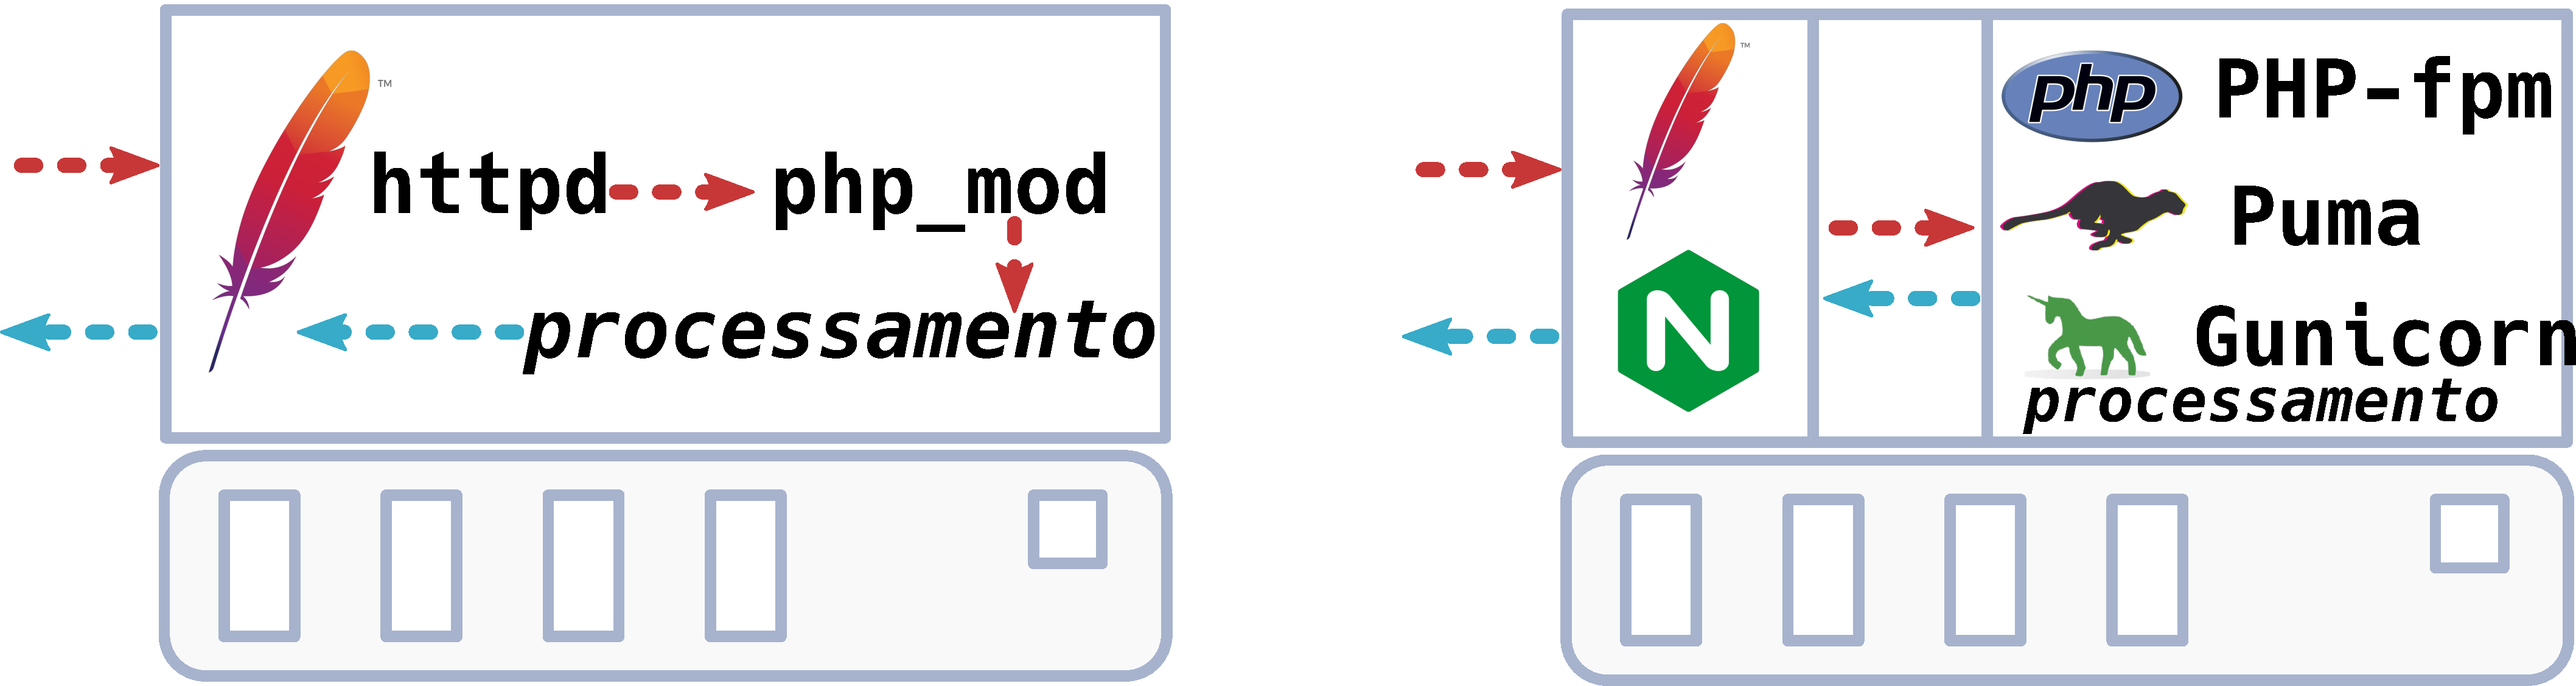
\includegraphics[width=.60\textwidth]{web_server_organization_strategy}
  \caption{Visão geral da organização de aplicações utilizando servidores Web}
\label{fig:web_server} \end{figure}

Atualmente podemos encontrar um grande número de arquiteturas que podem ser
utilizadas por um sistema web. A Figura \ref{fig:web_server} ilustra duas
arquiteturas diferentes. A primeira mostra uma situação na qual uma página web
é totalmente manipulada pelo Apache HTTPD. Basicamente, o HTTPD manipula uma
solicitação e passa ela para um módulo específico responsável por executar um
software (p.ex.: uma página web em PHP é executado por um módulo PHP chamado de
\emph{php\_mod}). A segunda arquitetura é um exemplo de página web escrita em
\emph{Ruby on Rails} que é composta de duas camadas: (1) um servidor web para
manipular as requisições que chegaram dos clientes (pode ser o Apache ou
Nginx), (2) um servidor de aplicação responsável por executar um programa (no
exemplo da figura, temos o PUMA que é especializado em executar código Ruby).
Esses exemplos, ilustram que podemos ter diferentes formas de organizar as
aplicações.

\begin{figure}[!h] \centering
  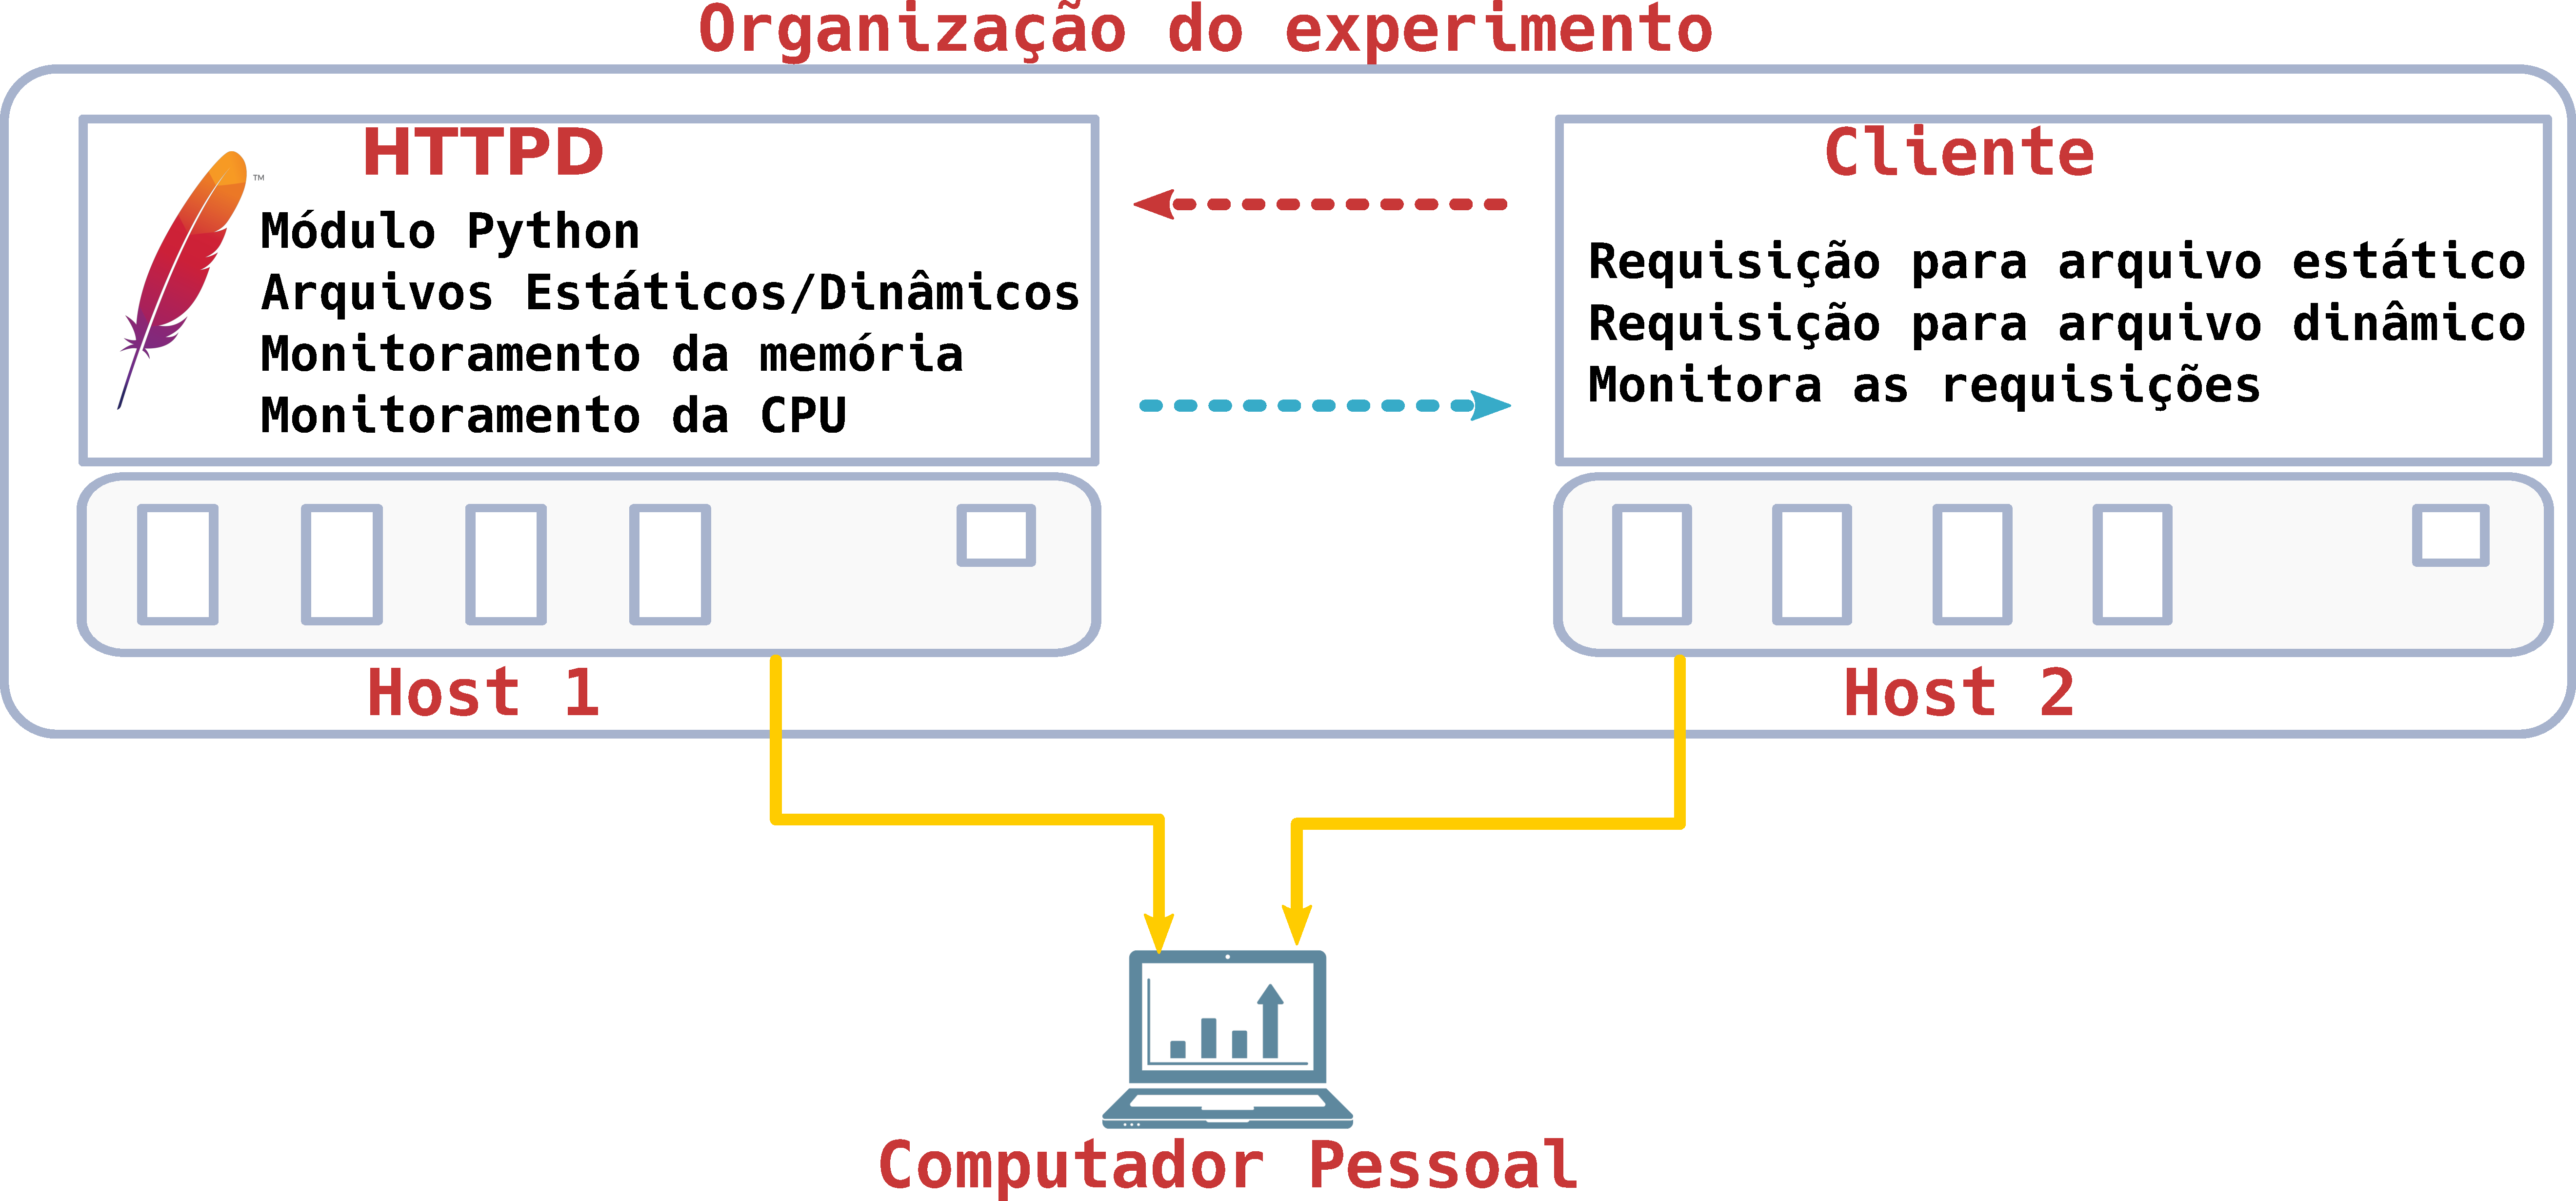
\includegraphics[width=.90\textwidth]{experiment_arhitecture}
  \caption{Arquitetura do experimento} \label{fig:experiment_architecture}
\end{figure}

A Figura  \ref{fig:experiment_architecture}, ilustra de forma geral a estrutura
utilizada para conduzir os experimentos com MVAS. Note que a figura indica duas
máquinas virtuais (Host 1 e Host 2), uma com um servidor web configurado para
dar suporte para uma grande carga de requisições geradas por uma segunda
máquina, que por sua vez, é responsável por simular um grande número de
clientes concorrentes. Ambas as máquinas são conectadas via conexão Gigabit
Ethernet, uma vez que queremos simular múltiplos cliente fazendo requisições
sem ter que se preocupar com questões de sobrecarga da rede.

Nos experimentos, nós queremos simular uma situação na qual o HTTPD terá que
lidar com uma grande carga que gere pressão na aplicação e assim eleve a
utilização de recursos de hardware. Com essa ideia em mente, nós conduzimos
dois experimentos empíricos com o objetivo de determinar qual seria a
configuração ideal para o Host 1. Primeiro, nós investigamos as principais
características das diferentes estrategias de MPM e notamos que o
\emph{Prefork} tem um grande consumo de memória; por isso, a quantidade de
memória foi escolhida com base no \emph{Prefork} uma vez que se espera que as
estratégias de \emph{Worker} e \emph{Event} consumam menos memória. Em segundo
lugar, nós conduzimos um pequeno conjunto de experimentos com diferentes cargas
de trabalho (\emph{workload}) e monitoramos a utilização de recursos. Nós
analisamos os \emph{logs} e concluímos que a forma mais rápida de tornar evidente a
diferença entre as estratégias é utilizando poucos núcleos e ter um bom
tamanho de memória. Consequentemente, nós decidimos utilizar uma máquina de
13GB de memória RAM e 2 núcleos. Note que 13GB é um tamanho selecionado visando
dar suporte para um grande número de requisições quando o HTTPD é configurado
para utilizar o \emph{Prefork}. Finalmente, é importante ressaltar que o Host 1
tem uma ferramenta configurada para monitorar a utilização de memória e CPU
(Collectl\footnote{\url{http://collectl.sourceforge.net/} Acessado dia 03/07/2018})
que é posteriormente recuperada para análise.

A segunda máquina, tem uma coleção de \emph{scripts} que utiliza a ferramenta de
Benchmark do Apache (ab) para gerar diferentes testes; a Figura
\ref{fig:experiment_architecture} ilustra a máquina que é responsável por
produzir diferentes cargas. Todas as requisições são monitoradas e salvas em
arquivos. Depois, todas as informações produzidas pela segunda máquina são
recuperadas e processadas.

\section{Customizações no Servidor Apache e no GNU/Linux}
\label{sec:customization}

Uma das principais características do HTTPD é a sua habilidade de ser
facilmente ajustado por meio de arquivos de configuração. Da perspectiva de um
usuário avançado, o Apache HTTPD pode ser mais flexível e adaptável para
diferentes contextos. Apesar de toda a flexibilidade e capacidade do HTTPD,
esse vem com uma configuração conservadora por padrão para evitar que os
usuários não experientes causem algum tipo de dano ao seu próprio ambiente.
Consequentemente, é necessário configurar o HTTPD para suportar grandes cargas
de requisições. Da mesma forma, o GNU/Linux também vem configurado de maneira
conservadora e esse também possibilita um elevado grau de personalização.
Portanto, um usuário avançado que desejar fazer com que o Linux entregue o
melhor desempenho possível para cada hardware, precisa personalizar vários
arquivos internos (em alguns caso, até recompilar o Kernel). Nesse trabalho,
nós queremos simular uma situação que se assemelhe a de um servidor web que
manipule uma elevada carga de requisições, por isso, fizemos diversas
otimizações no servidor Apache e no Linux.

Nos nossos experimentos, nós utilizamos e comparamos: \emph{Prefork},
\emph{Worker} e \emph{Event}. Todas as estratégias de MPM tem um arquivo de
configuração específico associado a si, na qual cada um permite algum tipo de
ajuste fino. Seguem os principais parâmetros disponíveis para configurar esse
tipo de MPM:

\begin{description}
  \item [StartServers:]
Espera um inteiro positivo que representa o total de processos que serão
iniciados junto com o HTTPD.  O valor padrão varia de acordo com o MPMs adotado
\citep{mpm_start_server};

  \item [MinSpareServers:]
Espera um inteiro positivo e ajusta o número mínimo de processos ociosos. É
importante ter um conjunto de processos desocupados para o caso em que o HTTPD
receba uma grande carga de requisições em um curto intervalo de tempo, os
filhos ociosos podem ser usados para tentar tratar as novas requisições. O
processo pai compara o total de filhos com o valor contido em
\textit{MinSpareServers}. Se tiver apenas alguns filhos ociosos, então o
processo pai cria novos filhos \citep{mpm_min_spare};

  \item [MaxSpareServers:]
Espera um valor positivo inteiro e configura o número máximo de processos
ociosos. Repare que \textit{MinSpareServers} e \textit{MaxSpareServers}
trabalham juntos controlando o total de recursos sendo utilizado pelos filhos
\citep{mpm_max_spare};

  \item [MaxRequestWorkers:]
Ajusta o número total de requisições servidas pelo HTTPD. Se o número total de
requisições é maior que o \textit{MaxRequestWorkers}, então toda nova
requisição será enfileirada. O tamanho da fila no Apache HTTPD é configurada no
parâmetro \textit{ListenBacklog} \citep{mpm_max_request};

  \item [ListenBacklog:]
Indica o tamanho máximo da fila.  Esse valor tem relação com o
tamanho da fila TCP definida pleo GNU/Linux \citep{mpm_listen};

  \item [ServerLimit:]
Eleva o número máximo de processos permitidos pelo HTTPDS
\citep{mpm_server_limit};

  \item [MinSpareThreads:]
Espera um inteiro positivo que representa o número mínimo de \emph{threads} ociosas.
Se tem muitas requisições para o servidor e não tem \emph{threads} ociosas o
suficiente para manipular toda a carga, o processo filho cria mais \emph{threads} até
que alcance um número de \emph{threads} maior do que o valor especificado nesse
parâmetro.  Por padrão, o HTTPD ajusta um valor de 75 para esse
parâmetro~\citep{mpm_minsparethreads};

  \item [MaxSpareThreads:]
Espera um inteiro positivo que representa o número máximo de \emph{threads} que podem
ficar ociosas. Se o HTTPD tem mais \emph{threads} ociosas do que o valor especificado
nesse parâmetro, então o processo pai mata os filhos excedentes. Por padrão,
esse valor é ajustado para 100 \citep{mpm_maxsparethreads};

  \item [ThreadLimit:]
Espera um inteiro positivo que representa um limite superior de \emph{threads} por
processo \citep{mpm_threadlimits};

  \item [ThreadPerChild:]
Espera um inteiro positivo que represente o total de thread por processo filho
\citep{mpm_threadperchild};

\end{description}

\begin{table}
  \centering
  \begin{tabular}{|c|c|c|c|}
  \hline
    \textit{Parameter} & \textbf{Event} & \textbf{Worker} & \textbf{Prefork} \\
      \hline\hline
    \textbf{ServerLimit} & 6000 & 6000 & 5000\\
      \hline
    \textbf{StartServer} & 10 & 10 & 1000\\
      \hline
    \textbf{MinSpareThreads} & 512 & 512 & --\\
      \hline
    \textbf{MaxSpareThreads} & 1024 & 1024 & --\\
      \hline
    \textbf{ThreadLimit} & 64 & 64 & --\\
      \hline
    \textbf{ThreadPerChild} & 64 & 64 & --\\
      \hline
    \textbf{MaxRequestWorkers} & 5120 & 5120 & 5000\\
      \hline
    \textbf{MinSpareServers} & -- & -- & 500\\
      \hline
    \textbf{MaxSpareServers} & -- & -- & 1500\\
      \hline
  \end{tabular}

  \caption{Configuração adotada para o MPM}
  \label{tab:configuration}

\end{table}



A Tabela \ref{tab:configuration}, ilustra as customizações que utilizamos para
configurar o HTTPD para os experimentos. Nossa configuração permite que o
Apache responda uma elevada quantidade de requisições o que torna o
experimentos próximo de uma situação realista. Nossas customizações no
GNU/Linux e HTTPD permite que boa parte do hardware seja utilizado.

\begin{table}
  \centering
  \begin{tabular}{|c|c|} \hline
  \textit{parameter} & \textbf{value}\\
    \hline\hline
   Max queue events & 1048576\\
     \hline
   Max user instances & 1048576\\
    \hline
   Max user watches & 1048576\\
    \hline
   Max map count & 262144\\
    \hline
   TCP max syn backlog & 8096\\
    \hline TCP syncookies & 0\\
    \hline
  \end{tabular}

  \caption{Configurações feitas no Kernel}
  \label{tab:kernel_config}
\end{table}



Também é necessário customizar o GNU/Linux uma vez que as configurações padrão
deste são feita para evitar o consumo de todos os recursos de hardware (p.ex.; o
Linux limita uma aplicação como o HTTPD). A Tabela \ref{tab:kernel_config}
mostra todas as configurações feita no GNU/Linux para esse experimento.
Observe que o GNU/Linux estabelece um limite de arquivos que podem ser abertos
por meio dos \emph{File Descriptor (FD)}, tal situação representa um problema
quando o HTTPD precisa manipular uma grande quantidade de requisições uma vez que cada uma
mantém um FD. Para superar esse problema, elevamos a quantidade
total de FDs suportados pelo Linux (Na Tabela \ref{tab:kernel_config}, o
parâmetro \emph{Max map count}), tal alteração permite que o HTTPD manipule um
maior número de requisições. Além disto, o GNU/Linux tem uma coleção de
arquivos de configuração que previnem alguns ataques de rede bem conhecidos. No
nosso caso, nós precisamos desabilitar o \emph{SYN Flood Protection} (Tabela
\ref{tab:kernel_config}, TCP syncookies) uma vez que essa configuração evita
que o SO manipule uma quantidade gigantesca de requisições feitas de uma mesma
máquina. Por fim, o tamanho padrão da fila TCP é pequena para esse estudo de
caso, portanto, nós elevamos consideravelmente o tamanho dessa (A Tabela
\ref{tab:kernel_config}, TCP max syn backlog, Max queue events, e Max user
instances).

Para concluir, nós fizemos ajustes finos no HTTPD e GNU/Linux para que esses
suportassem uma cargas de requisições elevadas. Essas configurações são
importantes para o contexto desses experimentos uma vez que desejamos por o
HTTPD sobre pressão para mostrar o comportamento do MVAS em tal situação.

\section{Cenários}

É comum encontrar aplicações rodando no HTTPD que também trabalhem com banco de
dado. Normalmente, esse tipo de aplicação tem que esperar para que uma
operação retorne algum tipo de dados. Esse cenário pode ser facilmente
expandido para uma situação na qual grandes quantidades de requisições são
feitas e o banco de dados fica ocupado. As vezes, os servidores de aplicações
também apresentam estrategias de cache, o que gera um cenário completamente
novo. Com essas questões em mente, é preciso decidir qual tipo de experimentos
queremos conduzir. Essa seção descreve os cenário adotados.

\subsection{Cenário Selecionado} \label{sec:scenarios}

\begin{table}[!h]
  \centering
  \begin{tabular}{|c|c|c|}
      \hline 
    & \textbf{Pequeno} & \textbf{Grande}\\
      \hline\hline
    Estático & 70Kb & 120Kb\\
      \hline
    Dinâmico & 80Kb & 120Kb \\
      \hline
  \end{tabular}

  \caption{Tamanho dos arquivos para serem transferidos}
  \label{tab:file_size}
\end{table}



Nossos experimentos foram compostos por dois cenários diferentes, separados por dois
tipos de arquivos: estático e dinâmico. Nós utilizamos dois arquivos estáticos
com texto puramente HTML de tamanhos distintos. A Tabela \ref{tab:file_size}
mostra os arquivos adotando, em especial, os tamanhos dos arquivos são baseados
em valores de um Relatório publicado em 2015 na qual indica que um arquivo HTML
tem em média 66KB. Para os arquivos dinâmicos, foi escrito
um pequeno código em Python que gera diferentes saídas por requisições. Nós
decidimos por essa estratégia com os arquivos dinâmicos para evitar os sistemas
de cache. Finalmente, os arquivos dinâmicos são importantes em um cenário em
que a CPU deve ser mantida ocupada por um período maior de tempo e com o
tamanho dos arquivos afetando nisto.

O HTTPD entrega arquivos estáticos HTML com pouca utilização de hardware uma
vez que esses arquivos não necessitam de processamento. Essas características
são desejáveis para mostrar a diferença entre o Prefork, Event e Worker ao se
utilizar o MVAS dentro do Apache Server com um tipo de requisição que demandam
pouca CPU. Por outro lado, os arquivos dinâmicos são utilizado para
experimentos que usam muita CPU e são usados para simular uma situação na qual
uma requisição tem que esperar por processamento. Essa situação gera sobrecarga
na CPU e consequentemente consome uma enorme quantidade de memória uma vez que
os processos vivem por mais tempo (até o fim do processamento).

\begin{table}[h!]
  \centering
  \begin{tabular}{|c|c|c|}
      \hline
    Casos & \textbf{Requisições} & \textbf{Concorrência}\\
      \hline\hline
    Arquivos estáticos & 60000 & 20000\\
      \hline
    Arquivos dinâmicos & 5000 & 600 \\
      \hline
  \end{tabular}
  \caption{Carga principal aplicada}
  \label{tab:loads}
\end{table}



A Tabela \ref{tab:loads} ilustra a carga aplicada nos experimentos. Para os
arquivos estáticos, nós aplicamos a maior carga de requisições com o maior
nível de concorrência; já para os arquivos dinâmicos, nós aplicamos uma carga
de requisições menor com pouca concorrência. Nosso objetivo com essas
configurações foi examinar em um ambiente sem alteração nas abstrações de
processos, qual a diferença em utilizar uma abordagem baseada em processos e
outras usando \emph{threads}. Tendo essa clara distinção entre as estratégias,
passamos a ter um cenário base para comparações com novos cenários que utilizam
alterações nas abstrações de processos. Por fim, vale observar que estamos
ignorando os casos com \emph{keep-alive}.

\section{MVAS Dentro do GNU/Linux e Apache HTTP Server}
\label{sec:mvas_inside_httpd}

O SpaceJMP \citep{spacejmp} foi a primeira implementação do conceito de MVAS e
está disponível para os SOs \emph{DragonFlyBSD} e \emph{Barrelfish}. Em 2016 os pesquisadores
envolvidos com o SpaceJMP decidiram implementar o MVAS no Kernel Linux com a
intenção de estender o trabalho original e enviar a modificação como uma
sequência de \emph{patches} para os mantenedores do Kernel. Como resultado, em
Agosto de 2016, foi lançado a primeira versão do MVAS para o Linux
\footnote{\url{https://github.com/l3nkz/linux/tree/mvas} Accessed at 2017/07/03} por
um dos pesquisadores.
 
Para utilizar a atual implementação do MVAS no Linux, nós trabalhamos em um
\emph{fork} feito da \emph{branch} original mantida pelo Till Smejkal (o
criador da implementação do MVAS no Linux). Durante nossos trabalhos, nós
tivemos que aprender como compilar, customizar e instalar a versão do Kernel
com MVAS. Para essas atividades, nós utilizamos o Debian com o Kernel fornecido
pelo Till.

MVAS é acessível por meio de chamadas de sistema e também possui algumas
informações que permitem auxiliar na depuração de problemas. Adicionalmente,
nós estudamos parte da implementação da MVAS para conseguir melhorar os
experimentos e também colaborar com o mantenedor. Durante muito tempo, a
pesquisa foi conduzida em conjunto com Till Smejkal, Ranjan Sarpangala e o
laboratório da HPe (responsáveis pela pesquisa). Contudo, tal implementação foi
abandonada temporariamente.
 
\subsection{MVAS Dentro do Apache HTTP Server}

Uma requisição tem um ciclo de vida curto dentro do HTTPD uma vez que é criada
e destruída frequentemente. As informações sobre um cliente e as suas conexões
são armazenadas dentro de uma estrutura de dados para manter as informações
sobre as requisições. Note, que da perspectiva da segurança, é desejável
adicionar o maior nível de isolamento possível para cada requisição. A forma
como as requisições devem ser tratadas devem ser leves, do contrário não poderá
ser utilizado em uma aplicação como o HTTPD. Embora o modelo baseado em
processos isole todas as requisições mantendo um desempenho aceitável, esse
gera um grande consumo de memória (Seção \ref{sec:prefork}).  Por outro lado, a
estratégia baseada em \emph{thread} tem melhor desempenho mas não
proporciona um isolamento completo uma vez que parte da memória é compartilhada
com outras \emph{threads}.

O modelo do MVAS tem um mecanismo para criar múltiplos espaços de endereçamento
virtual, todos inteiramente isolados e com um comportamento que gera
persistência de dados (Seção \ref{sec:mvas}). Nossa hipótese sobre a utilização
do MVAS era a de que esse poderia ser utilizado como uma solução híbrida na
qual fornecesse o mesmo nível de isolamento de um processo com um desempenho
aproximado ao das \emph{threads}. Com tal ideia em mente, nós alteramos o ciclo
de vida das requisições do Apache com a intenção de verificar a nossa hipótese.

\begin{figure}[!h]
  \centering
  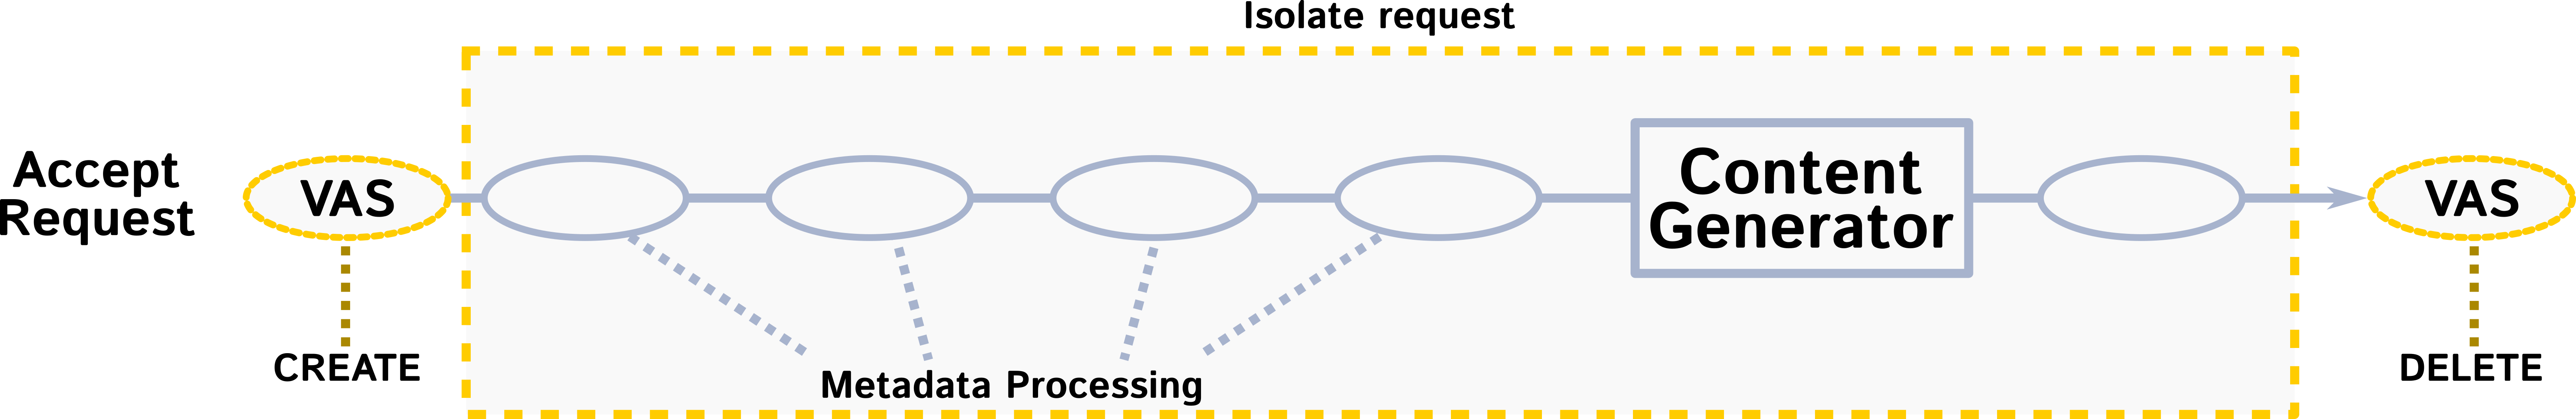
\includegraphics[width=\textwidth]{mvas_httpd}
  
  \caption{HTTPD com MVAS}
  \label{fig:httpd_mvas}
\end{figure}

A Figura \ref{fig:httpd_mvas} mostra a nossa abordagem para adicionar o MVAS
dentro do HTTPD. Antes da estrutura de dados da requisição ser construída no
Apache HTTPD, nós temos que criar uma nova VAS, anexar ela na \emph{thread}
atual e mudar para a nova VAS. Depois, todo o ciclo de vida da requisição vai
ser realizada da forma usual, mas dentro de uma nova VAS (totalmente isolada).
Quando uma requisição termina, procedemos com a limpeza das informações
relacionadas a VAS. Essa abordagem garante o total isolamento de qualquer
requisição.

Nós identificamos as exatas funções que mantém todo o ciclo de vida de um
requisição e aplicamos MVAS para isolar. Essas funções são:

\begin{quote}
  \texttt{process\_http\_async\_connection} e\\
  \texttt{ap\_process\_http\_sync\_connection} (ambas localizadas no arquivo
  \texttt{modules/http/http\_core.c})
\end{quote}

Os módulos MPM invocam uma dessas funções para manipular um ciclo de vida de
uma requisição, por esse motivo, adicionar MVAS nessas funções elimina a
complexidade relacionada ao código. Contudo, adicionar o MVAS eleva a
sobrecarga geral para atender as requisições.

O Código \ref{lst:http_core} é um pedaço extraído de uma implementação do MVAS
dentro do Apache HTTPD. Repare que a função \texttt{create\_isolate\_vas()} é
projetada para dar suporte para a criação de uma nova VAS dentro do Apache
HTTP. O código também chama as funções
\texttt{ap\_process\_http\_async\_connection} e
\texttt{ap\_process\_http\_sync\_connection}, ambas isoladas dentro de uma nova
VAS. No começo de cada uma dessas funções é criado uma nova VAS, anexada ao
processo atual e finalmente mudada para uma nova VAS depois que o HTTPD cria a
requisição. No fim do ciclo de vida, nós removemos a VAS. Nossa implementação
ainda precisa de melhorias, mas já é funcional. Finalmente, todo o código fonte
das nossas modificações está disponível no Github em
\url{https://github.com/LSS-USP/httpd-experiment/tree/mvas\_worker}.

\begin{ruledcaption}{Alteração no Apache Server\label{lst:http_core}}
\lstinputlisting[
    language=C,
    ] {code/http_core.c}
\end{ruledcaption}

Nós esperamos que o MVAS adicione mais latência, contudo, nós queremos
investigar se a sobrecarga extra é tolerável ou não. O objetivo principal desse
experimento é verificar se o MVAS pode ser utilizado como uma substituição a
estratégia baseada em processos.

\section{Resultados}
\label{sec:preliminary}

O método proposto na Seção \ref{sec:metodologia} busca evidência de forma
clara, sistemática e replicável as diferenças entre as estratégias baseadas em
processos e \emph{threads}. Por isso o primeiro passo desses experimentos consiste em
deixa claro a diferença entre as estratégias de MPM, para que em seguida, com
os resultados e a estrutura utilizada, possamos expandir os experimentos para a
versão do Apache que utiliza MVAS.

\subsection{Existe Alguma Diferença Significativa de Desempenho Entre o Apache
HTTP Trabalhando com Processos e Threads?}

Nesse primeiro cenário, nós temos o HTTPD com as alterações explicadas na Seção
\ref{sec:customization}, mas sem as modificações do MVAS. Responder essa
pergunta traz vantagens: (1) deixa claro a diferença entre processos e \emph{threads}
no Apache, (2) temos o comportamento base para comparar com o MVAS e (3)
validamos a nossa metodologia.

\begin{table}[h!]
  \centering
  \begin{tabular}{|c|c|c|}
      \hline
    Nome & \textbf{Núcleo} & \textbf{Memória}\\
      \hline
    M1 & 2 & 13Gb \\
      \hline
    M2 & 2 & 4Gb \\
      \hline
   \end{tabular}

  \caption{Hardware}
  \label{tab:machines}
\end{table}



Na Seção \ref{sec:metodologia} e \ref{sec:scenarios}, detalhamos a nossa
metologia e a configuração básica que seguimos. Duas máquinas foram utilizadas,
uma chamada de M1 e a outra de M2 como a Tabela \ref{tab:machines} mostra.
Repare que nós decidimos utilizar apenas alguns núcleos e memórias grandes uma
vez que essas condições são melhores para revelar o comportamento do HTTPD.

\begin{figure}[!h]
  \centering
  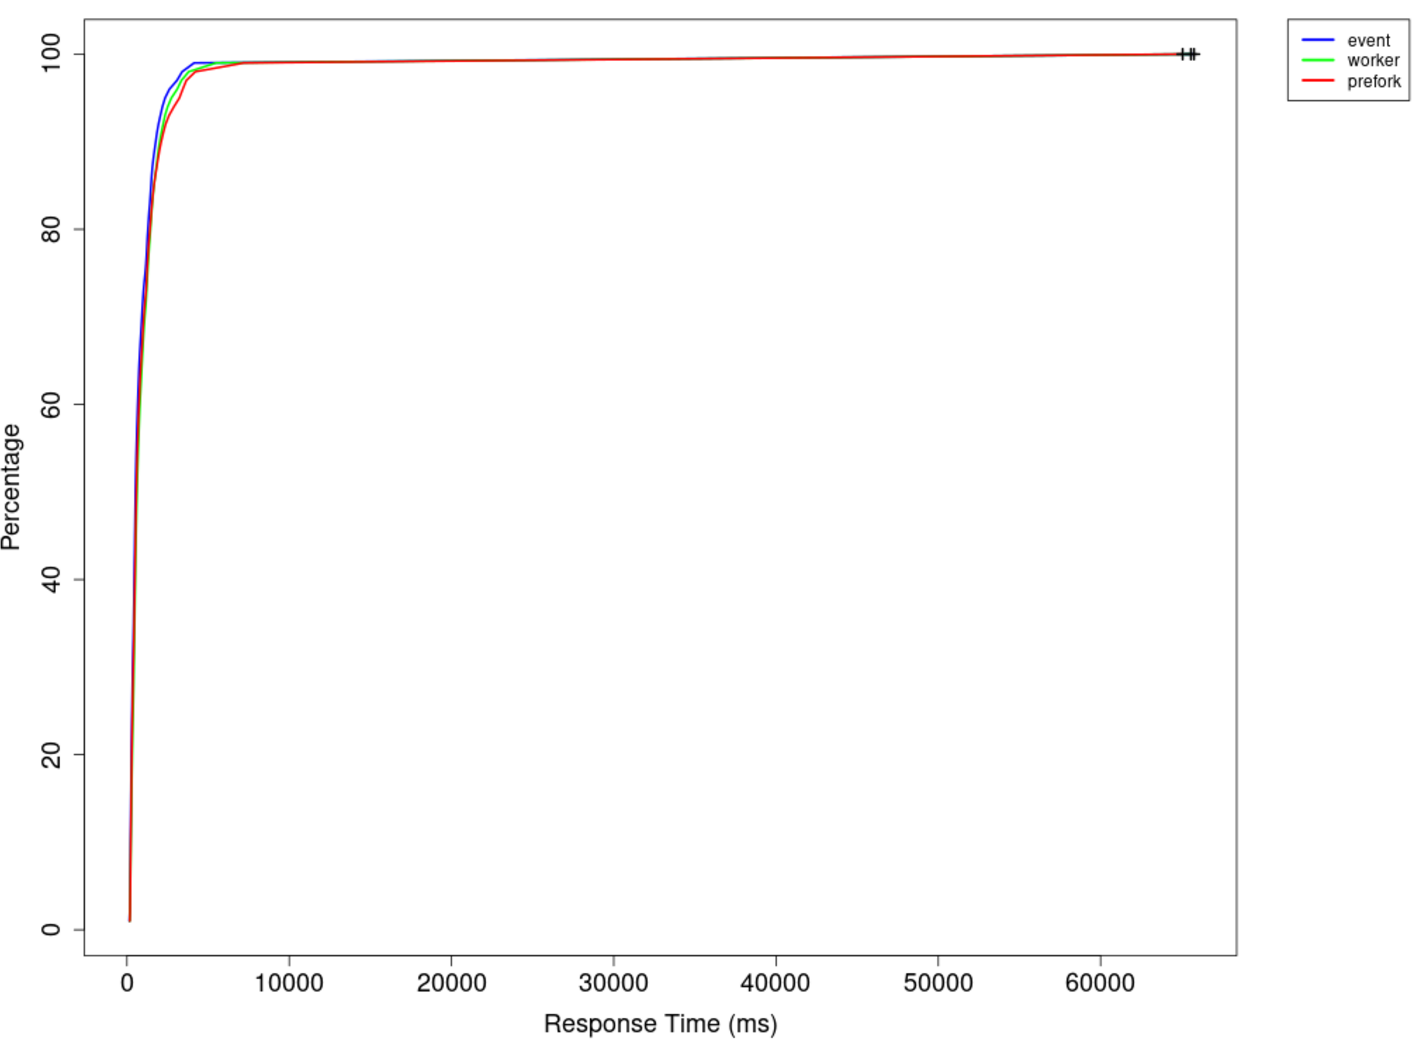
\includegraphics[width=.90\textwidth]{static_file}

  \caption{Arquivos estáticos: tempo gasto para servir o percentual de requisições}
  \label{fig:static_file}
\end{figure}

O gráfico na Figura \ref{fig:static_file} mostra o percentual de requisições no
eixo y; no eixo x temos o tempo gasto para atender o percentual de requisições
\citep{apache_ab}. A Figura \ref{fig:static_file} mostra o cenário na qual são
servidos arquivos estáticos que manipulam 60000 requisições simulando 20000
requisições em paralelo. Além disso, o gráfico ilustra o \emph{Prefork},
\emph{Worker} e \emph{Event} juntos para tornar mais simples de visualizar a
diferença.

\begin{figure}[!h]
  \centering
  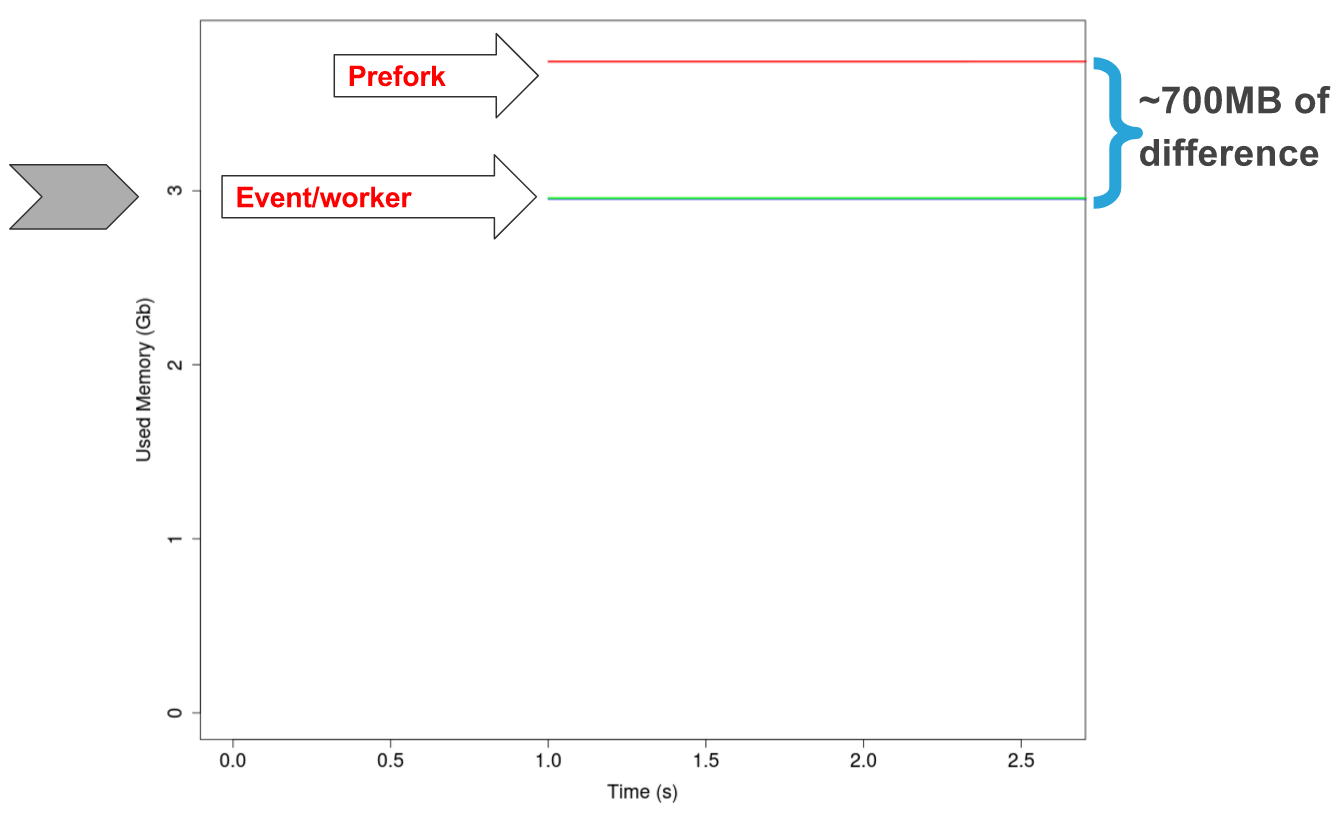
\includegraphics[width=.90\textwidth]{static_file_memory_usage}

  \caption{Arquivos estáticos: O consumo de memória necessário para atender todas as requisições}
  \label{fig:static_file_memory}
\end{figure}
 
Analisando a Figura \ref{fig:static_file}, é possível perceber que o tempo de
resposta foi praticamente o mesmo para todas as estratégias. Em uma primeira
análise, esse resultado pode parecer frustante uma vez que é de se esperar que
o \emph{Prefork} responda um número menor de requisições. Contudo, a Figura
\ref{fig:static_file_memory} apresenta o mesmo experimento sob a perspectiva do
consumo de memória. Repare que o \emph{prefork} utiliza aproximadamente 3.7Gb e
o \emph{event/worker} precisam de 3Gb para atender a todas as requisições. Esse
resultado evidência uma desvantagem do \emph{prefork} em um cenário simples.
Por fim, é importante ressaltar que um dos motivos de \emph{threads} e
processos terem o mesmo tempo de resposta nesse cenário vem do fato de que a
troca de contexto para \emph{threads} e processos é o mesmo no GNU/Linux
\citep{love}.

\begin{figure}[!h]
  \centering
  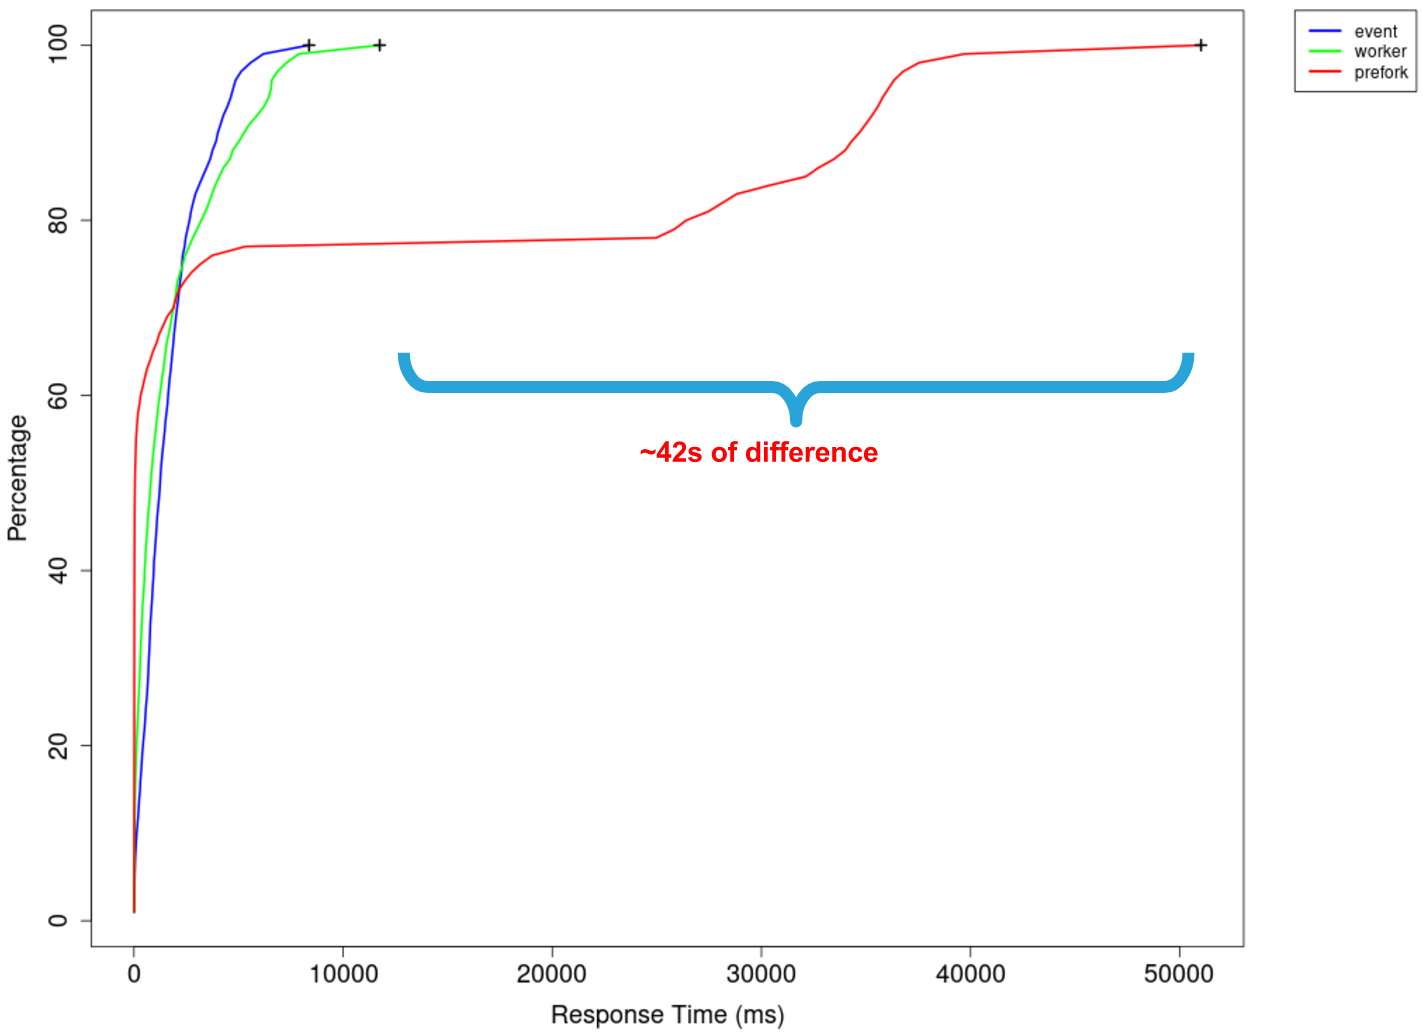
\includegraphics[width=.90\textwidth]{dynamic_file_request_time}

  \caption{Arquivos Dinâmicos: Tempo gasto por percentual de requisições}
  \label{fig:dynamic_file}
\end{figure}

\begin{figure}[!h]
  \centering
  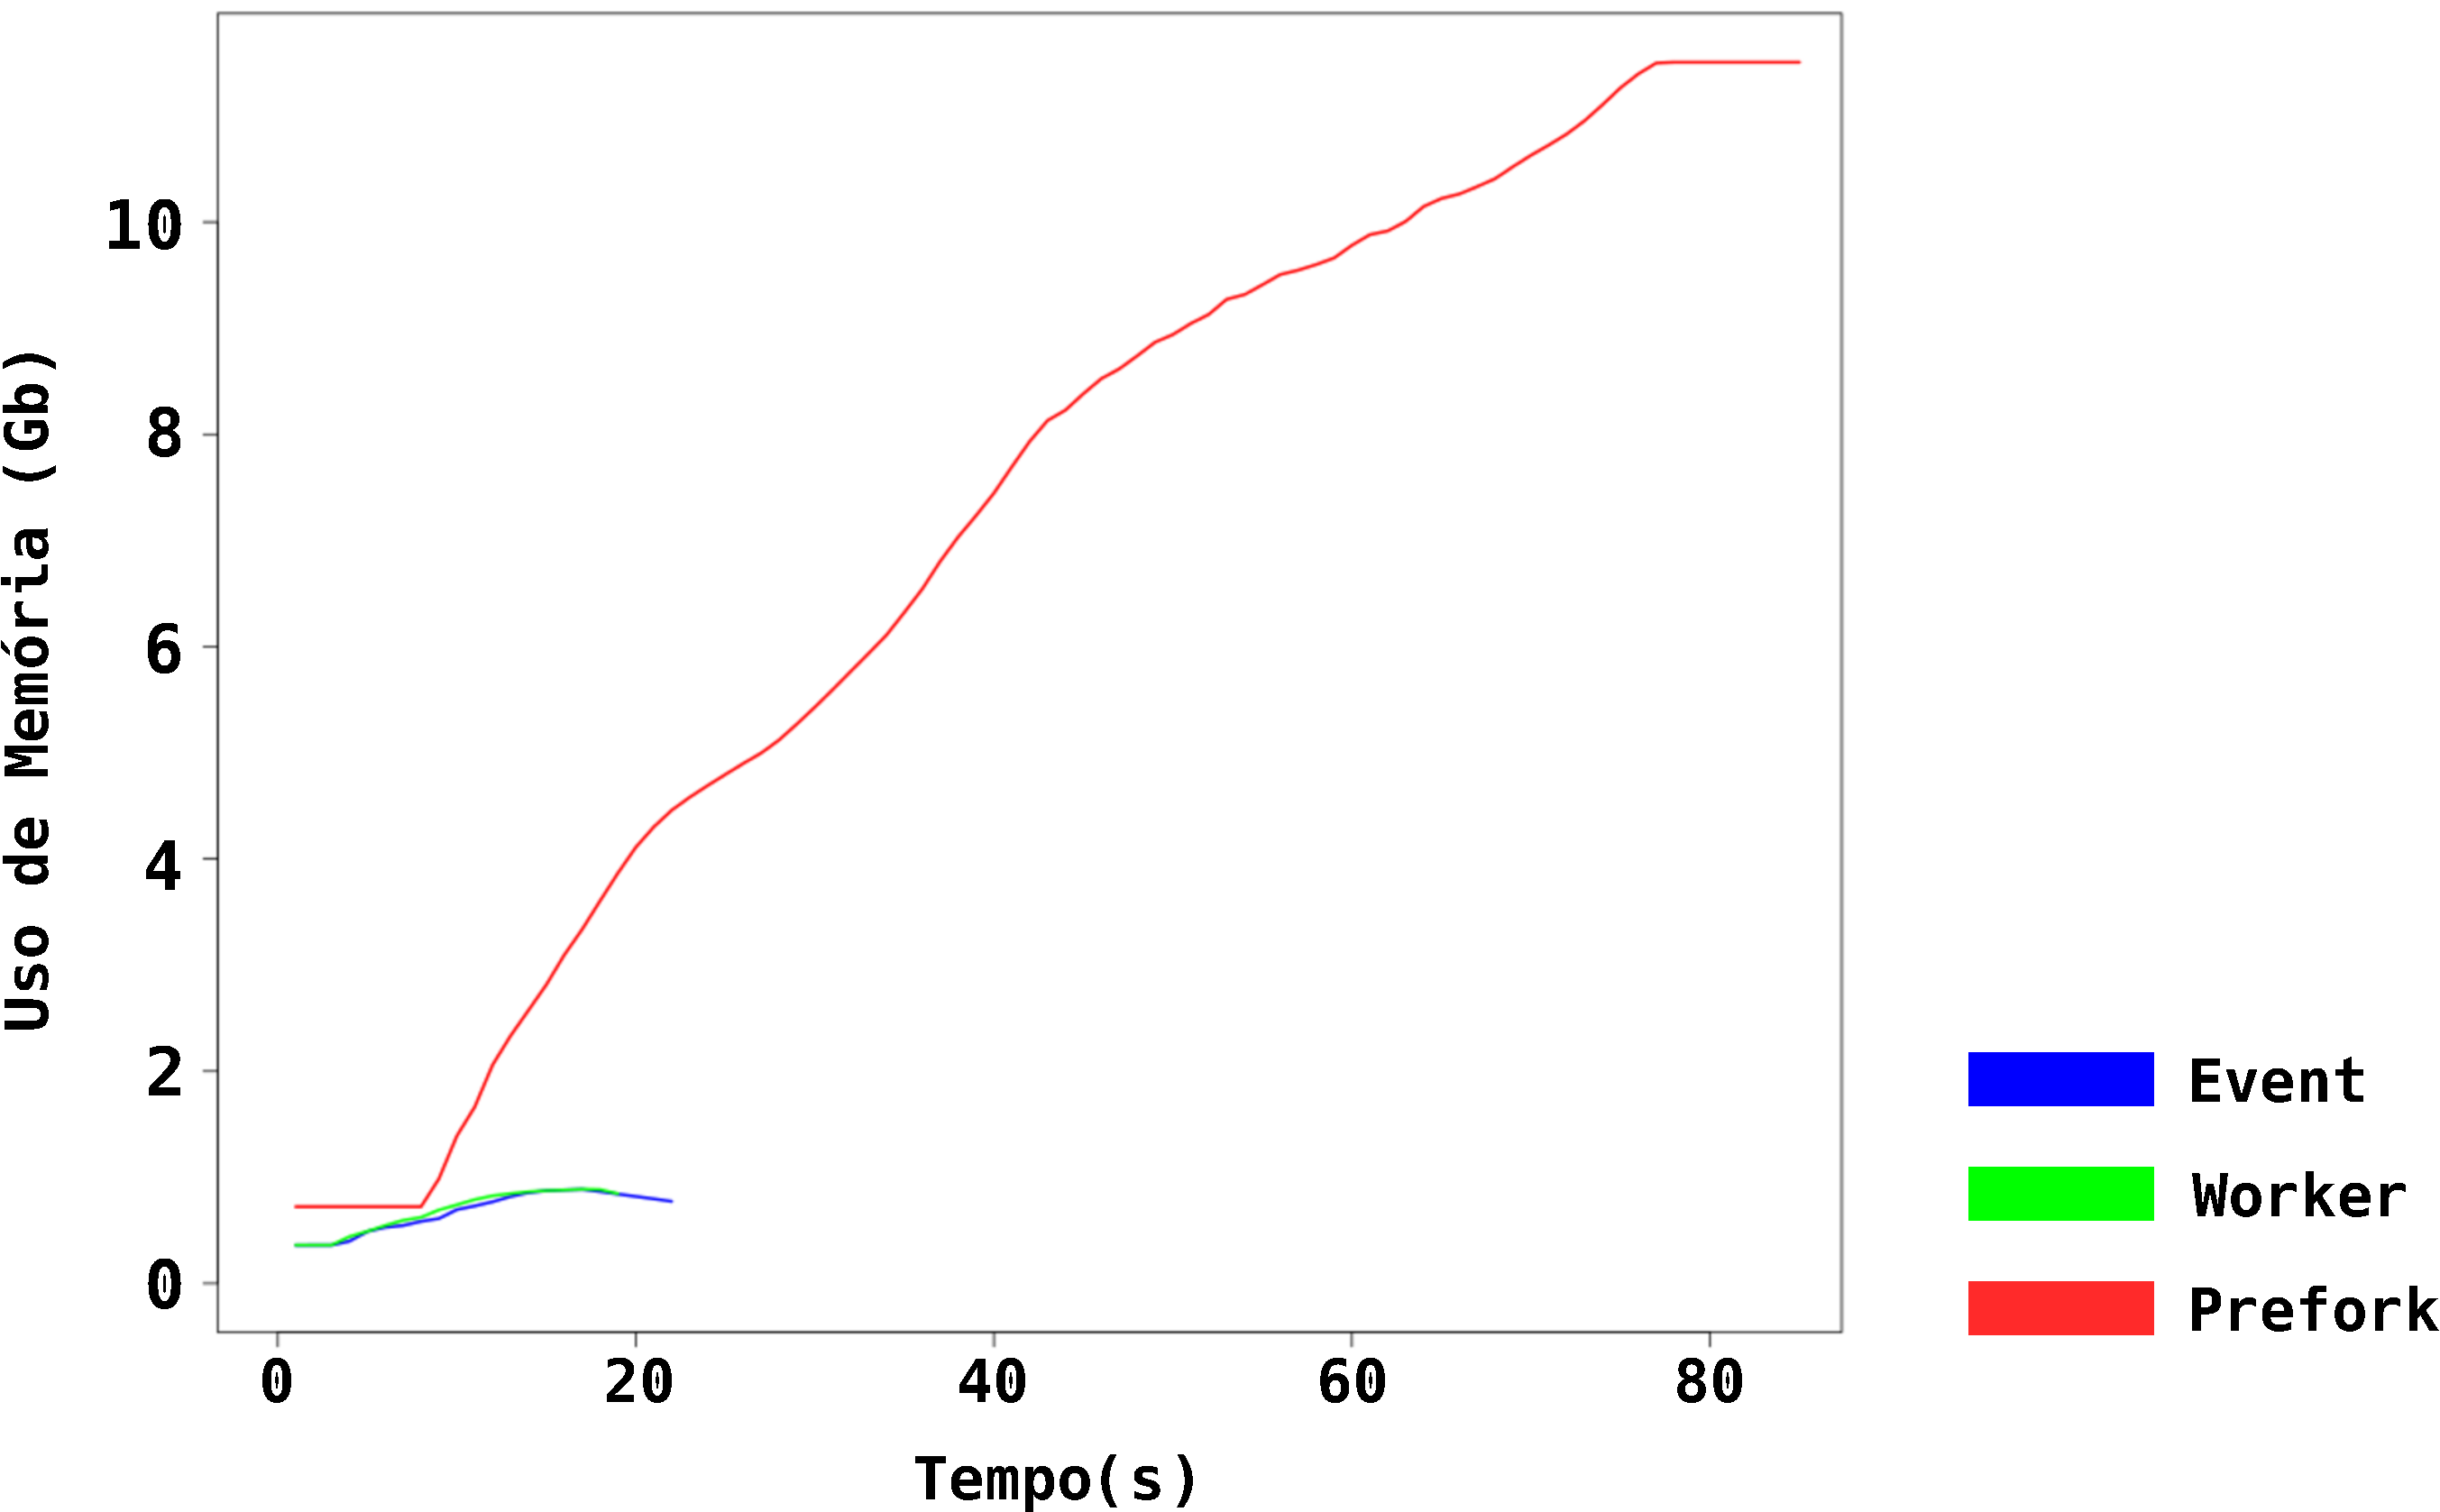
\includegraphics[width=.90\textwidth]{dynamic_file_memory_usage}

  \caption{Arquivos Dinâmicos: Consumo de memória necessário para servir as requisições}
  \label{fig:dynamic_file_memory}
\end{figure}

A Figura \ref{fig:dynamic_file} mostra um cenário com arquivos dinâmicos. Nesse
caso, a diferença entre processos e \emph{threads} são muito mais claras. O
\emph{prefork} é muito mais lento do que o \emph{Event} e \emph{Worker}, a
diferença é próxima de 42 segundos o que é inaceitável em um cenário real.
Para entender melhor esse caso, a Figura \ref{fig:dynamic_file_memory} mostra o
consumo de memória e explicita o enorme gasto de memória do \emph{prefork}
quando comparado com o \emph{Event} e \emph{Worker}. Essa situação pode ser
examinada da perspectiva do SO, basicamente o Apache tem que criar muitos
processos filhos por requisição e manter eles vivos até que o processamento
termine. Consequentemente, o Apache tem um enorme número de processos vivos e
consumindo memória. Por outro lado, \emph{threads} compartilham dados com os
processos pai o que reduz o total de memória gasta, assim, mantendo as
\emph{threads} vivas com um custo menor.

Podemos concluir que os experimentos tornam claro as diferenças entre processos
e \emph{threads} dentro do HTTPD. Os dois cenários descritos são suficientes
para servir como critério para mostrar a diferença entre os MPMs. O atual
resultado fornece informações básicas necessária para o restante dos
experimentos.

\subsection{Qual a Diferença de Desempenho do Apache Utilizando MVAS Quando
Comparado com as Estratégias Baseadas em Processos e \emph{Threads}?}

A segunda parte das validações tiveram como principais objetivo estudar o
comportamento do kernel Linux com MVAS e com o Apache fazendo uso dos seus
recursos. Como explicado na Seção \ref{sec:mvas_inside_httpd}, nós já temos a
versão modificada do HTTPD utilizando MVAS. Nós instalamos a versão do HTTPD e
executamos o \emph{benchmark} novamente. Contudo, nossos experimento apontaram
três problemas: (1) MVAS não funciona bem com múltiplas \emph{threads}, (2)
existem problemas de alocação de memória e (3) existe uma enorme sobrecarga nas
operações do MVAS.

Para o primeiro problema, nós conversamos diretamente com o autor do MVAS para
tentar identificar o que estava acontecendo. Depois de várias verificações na implementação,
o autor detectou problemas nas heurísticas de manipulação dos segmentos de
memória.  Basicamente, MVAS tem problemas relacionados a alocação de
pilha; infelizmente, resolver esse problema requer mudar praticamente
toda a implementação atual do MVAS.

Para o segundo problema, é preciso recorrer a fundamentação teórica e revisitar
como o Linux aloca memória. Na Seção \ref{sec:visao_pratica_mem} discutimos o
processo de alocação da memória em sistemas Linux e na Figura
\ref{fig:malloc_linux} ilustramos o segmento \emph{heap} para um programa.
Repare da primeira parte da Figura \ref{fig:malloc_linux} que o \emph{heap} é
mapeado para a memória física. Em seguida, o programa pede por mais memória
para o SO por meio da função \texttt{malloc()}. O Linux então estende o tamanho
do \emph{heap} e retorna uma nova referência para a memória imediatamente e
então espera que o programa tente escrever algo na memória.  Assim, depois de
uma tentativa de escrita na memória o kernel realmente aloca memória física
para o programa. Com essa ideia em mente, é possível perceber que o MVAS tem
que manipular esse tipo de situação e esse é um problema complicado para o MVAS
resolver. Infelizmente, o MVAS falha em mapear essa situação e cada mudança no
VAS, o SO perde a referência para a memória física.

\section{Discussão Sobre os Experimentos}

Durante a análise das diversas propostas de ampliação das abstrações de
processos, notamos que os dois principais métodos de validação consistem em
utilizar aplicações e \textit{microbenchmarks}. Como já discutimos no Capítulo
\ref{cap:validacoes}, o uso de aplicações é desejável uma vez que essas podem
ser amplamente utilizadas para verificar o impacto geral de uma modificação nas
abstrações de processos. Apesar de vários pesquisadores terem feito uso de tal
abordagem, notamos que nenhum deles realizou experimentos utilizando cargas
expressivas. Por exemplo, os trabalhos que alteraram o Apache realizavam testes
com algumas poucas dezenas de requisições para arquivos estáticos. Tais testes
não evidenciam a real natureza da alteração feita na abstração de processo pois
a aplicação modificada não é demandada de forma a exercitar o sistema.

Esta pesquisa surgiu de uma parceria com a HPe que tinha por objetivo levar o
SpaceJMP para o Kernel Linux por meio do MVAS. Para isso era necessário
demonstrar que o MVAS funcionaria bem no Linux, por isso ficamos responsáveis
de trabalhar nas validações de tal técnica. Como demostrado ao longo deste
capítulo, tal técnica não é escalável da forma como foi feita. Isso é
interessante de se observar uma vez que tal resultado dialoga com a
argumentação construída no Capítulo \ref{cap:validacoes}; por meio do uso de
aplicação foi demonstrado que uma nova abstração pode não escalar em um sistema real.
Note que esse resultado não significa que desacoplar a VAS é uma ideia ruim,
apenas ilustra que os estudos referentes a tal ideia ainda precisam avançar.

Durante este trabalho também buscamos replicar os resultados apresentados pelo
Dune; nós também colaboramos com os pesquisadores por meio do envio de
\textit{patches}. Os \textit{microbenchmarks} apresentados pelos pesquisadores
comportam-se perfeitamente como reportado, mas não foi possível replicar os
resultados com as aplicações pois parte do código não estava mais disponível. O
Dune é uma das propostas com maior potencial de ser incorporada nos SOs
modernos, contudo a sua implementação é insegura e não escalável. O principal
motivo para isso está no fato do Dune interceptar os endereços das chamadas de
sistemas. Tal abordagem não funciona desde o momento que o Kernel adotou o
sistema de randomização dos endereços de chamadas conhecido por
KASLR~\citep{kaslr}.

Portanto o principal objetivo desses capítulo era apresentar evidências e uma
visão prática da validação de uma nova abstração de processo usando uma
aplicação amplamente conhecida. Além disso, buscamos deixar claro a importância
em utilizar cargas de testes relevantes.
